\begin{frame}[fragile]{Stellingen en Bewijzen (Bewijzen)}
    Het invoegen van een \textbf{bewijs} is erg makkelijk als je \texttt{amsthm} hebt geïmporteerd. 
    \begin{minted}[highlightlines={6,8}]{tex}
        \documentclass{article}
        \usepackage[dutch]{babel}
        \usepackage{amsthm}
        \newtheorem{stelling}{Stelling}
        \begin{document}
        \begin{proof}
            Dit is mijn bewijs. 
        \end{proof}
        \end{document}
    \end{minted}
    \pause 
    Je krijgt dan:
    \begin{tcolorbox}[boxrule=0.5pt, colback=white]        
    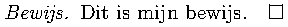
\includegraphics[width=0.3\textwidth]{Standalones/theorems_proofs_standalone.pdf}
    \end{tcolorbox}
\end{frame}

\begin{frame}[fragile]{Stellingen en Bewijzen (Bewijzen)}
    De taal waarin het woord `Bewijs' staat, hangt af van de \texttt{babel} package. 
    
    Als je \mintinline{tex}{\usepackage[english]{babel}} gebruikt, dan zal er 
    `\emph{Proof.}' staan. 
    \pause
    \begin{minted}[highlightlines={2}]{tex}
        \documentclass{article}
        \usepackage[dutch]{babel}
        \usepackage{amsthm}
        \newtheorem{stelling}{Stelling}
        \begin{document}
        \begin{stelling}
            Dit is mijn stelling
        \end{stelling}
        \begin{proof}
            Dit is mijn bewijs. 
        \end{proof}
        \end{document}
    \end{minted}
\end{frame}